\documentclass[11pt,a4paper,oneside]{article}


\usepackage[T2A]{fontenc}
\usepackage[utf8]{inputenc}
\usepackage[english,russian]{babel}
\usepackage[russian]{olymp}
\usepackage{graphics}
\usepackage{wrapfig}
\usepackage{amsmath}
\usepackage{amssymb}
\usepackage{epigraph}
\usepackage{graphicx}
\usepackage{multicol}


\newcommand{\qo}{\textquotesingle}
\newcommand{\qq}{\textquotesingle~}

\contest{ACM ICPC Kyrgyzstan Subregional 2015}{Бишкек}{1 ноября 2015 года}    

\binoppenalty=10000
\relpenalty=10000
\exhyphenpenalty=10000

\renewcommand{\t}{\texttt}

\createsection{\Note}{Примечание}

\renewcommand{\defaultmemorylimit}{256 мегабайт}

\begin{document}

\begin{problem}{Задача B. Фермер}{1 секунда}{256 мегабайт}

Пришла осень, и фермер Майрамбек решил посчитать, какой урожай пшеницы он может собрать со своих полей. У Майрамбека есть участок прямоугольной формы, разбитый на квадратные ячейки. На участке расположены  поля пшеницы. Пример расположения полей пшеницы показан на Рис. 1. 


\begin{figure}[ht]
\centering
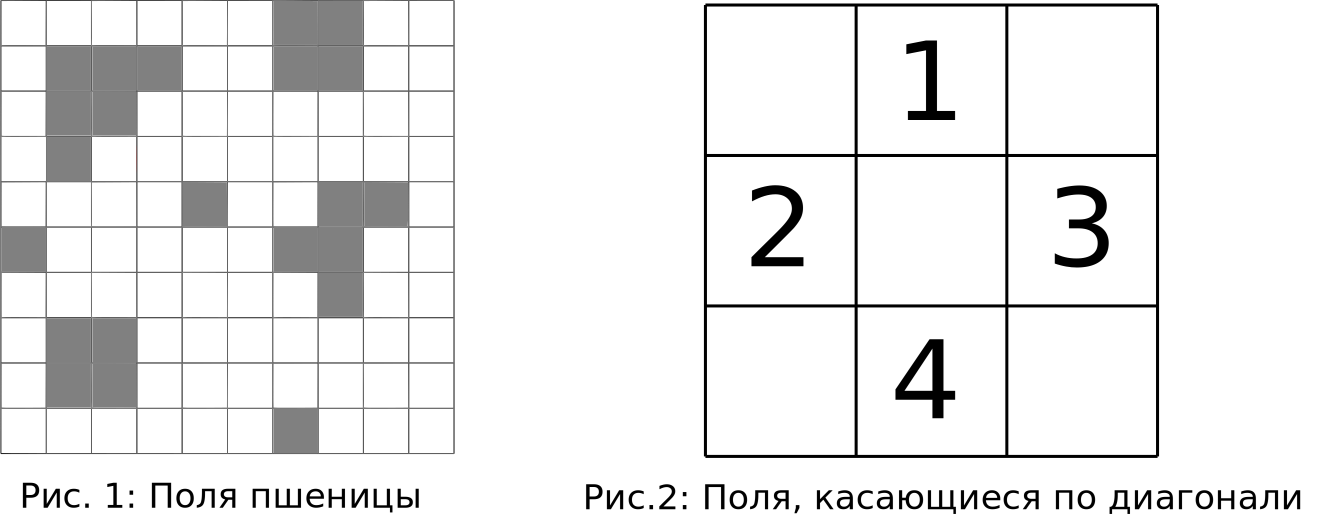
\includegraphics[width=0.8\textwidth]{pic2.pdf}
\end{figure}


Каждое поле представляет собой область, ограниченную краем участка и/или незасеянными ячейками. Граница поля – это незасеянные ячейки по вертикали и  горизонтали от крайней засеянной ячейки. Области, касающиеся только по диагонали (как на рисунке Рис. 2) считаются различными полями.  


На одном поле может быть  засеяно один или больше сортов пшеницы. Майрамбек хочет узнать, на каком поле, какой сорт сколько площади занимает. С помощью беспилотника Майрамбек сделал съемку своего участка, а сканер определил сорт пшеницы на каждом квадрате, и незасеянные квадраты.  Надо помочь Майрамбеку посчитать количество полей и для каждого поля – какую площадь занимает каждый из сортов пшеницы.

\InputFile
В первой строке два целых числа $M$ и $N$ – общий размер участка $(1 \leq N,M \leq 1000)$. В последующих M строках – план самого участка с полями. Каждая строка содержит $N$ чисел, которые описывают каждую ячейку строки. Если ячейка засеяна сортом пшеницы, то она отлична от нуля и содержит номер сорта пшеницы. Номер может быть целым числом от $1$ до $100$. Незасеянная ячейка содержит $0$. Полей не может быть больше $100$ и меньше $1$.



\OutputFile
Требуется вывести информацию о каждом засеянном поле в виде:

\begin{verbatim}
A1
C1 Sa11
…
CN Sa1N
…
AK
C1 SaK1
…
CN SaKN
\end{verbatim}




\begin{figure}[ht]
\centering
\includegraphics[width=0.45\textwidth]{drawing3.pdf}
\end{figure}

$Ak$ – номер поля. Поля нумеруются целыми числами от $1$ до $100$ последовательно, меньший номер имеет то поле, у которого номер строки самой верхней ячейки поля меньше, а при равенстве строк, меньший номер должно иметь то поле, у которого номер ряда самой левой ячейки в верхней строке меньше. На Рис. 3 показан пример нумерации полей пшеницы – темным цветом (зеленым) отмечены ячейки полей, по которым происходит сортировка. После, идут в порядки возрастания, номера сортов, засеянных на этом поле, и через пробел, площадь, занимаемая этим сортом пшеницы на поле.
На Рис. 3 (продолжение примера с Рис. 1) написаны только номера полей (не сорта пшеницы)


\Examples

\begin{example}%
\exmp{
5 5
0 0 0 1 0
0 2 2 2 0
0 1 3 4 0
0 0 0 0 0
0 1 3 2 0
}{
1
1 2
2 3
3 1
4 1
2
1 1
2 1
3 1
}%
\exmp{
10 10
0 0 0 1 1 1 1 1 0 0
0 0 0 1 0 0 0 1 0 0
0 0 0 1 0 2 0 1 0 0
0 0 0 1 0 1 0 2 0 0
0 0 0 0 2 2 2 0 0 0
0 0 0 0 3 3 3 0 0 1
0 1 1 1 0 0 0 0 0 0
0 1 1 1 0 0 0 0 0 0
0 1 1 1 0 0 0 0 0 0
0 0 0 0 0 0 0 0 0 0
}{
1
1 10
2 1
2
1 1
2 4
3 3
3
1 1
4
1 9
}%
\end{example}



\vspace{1.0cm}
\hfill \textit{Автор задачи: Беляев Aртем}
\medskip\noindent




\end{problem}


\end{document}
%%% Local Variables:
%%% mode: latex
%%% TeX-master: t
%%% End:
